
\chapter{Descripción Microprocesadores Disponibles en el Mercado}
	\section{Microprocesadores Soft-Core}
	Un microprocesador soft-core o abreviado SCP, es un microprocesador que puede implementarse utilizando síntesis lógica en diferentes dispositivos lógicos programables como CPLDs o FPGAs, o incluso puede incluirse en un diseño para ASIC.
 	Suelen distribuirse en forma de código fuente en algún lenguaje de descripción de hardware, principalmente VHDL o Verilog, aunque algunos SCPs
 	comerciales se distribuyen en formatos propietarios.
	Los principales fabricantes de dispositivos lógicos programables, como se dijo en capítulos anteriores, tienen su propio  SCP comercial especialmente
	diseñado y optimizado para funcionar en sus FPGAs. Así Xilinx tiene PicoBlaze \cite{Etiqueta15} y MicroBlaze \cite{Etiqueta16}, Altera
	proporciona Nios II \cite{Etiqueta17}, y Lattice distribuye LatticeMico32 \cite{Etiqueta18}. También existe una gran variedad de SCPs
	distribuidos en forma de código abierto, como el OpenRISC 1200 \cite{Etiqueta19} mantenido por la comunidad Opencores \cite{Etiqueta20}, o los  SCPs
	LEON2 y LEON3 \cite{Etiqueta21} \cite{Etiqueta22} que proporciona la compañía Gaisler Research \cite{Etiqueta23}.
		
	A continuación se presentan más detalladamente las características de estos SCPs%, y un resumen comparativo de sus características
	\subsection{PicoBlaze}
	
	PicoBlaze es un microcontrolador RISC de 8 bits desarrollado por Xilinx y optimizado para sus FPGAs. Esta optimizado para ocupar muy poco área y en cuanto a velocidad puede llegar a ejecutar entre 44 y 100 millones de instrucciones por segundo(MIPS), dependiendo del speedgrade y la familia de FPGA sobre la que se implemente. Las principales características de PicoBlaze son:
	
  
	\begin{itemize}
	  \item  16 Registros de propósito general de 1 byte.
	  \item 1024 bytes de instrucciones en memoria on-chip que se cargan al programarse la FPGA.
	  \item 256 puertos de entrada y 256 de salida para conectar lógica o periféricos externos.
	\end{itemize}
	
	La arquitectura general consiste en una serie de bloques presentados en la figura ~\ref{fig:PicoBlazer}.
		
	\begin{figure}[h!]
 	\begin{center}
  	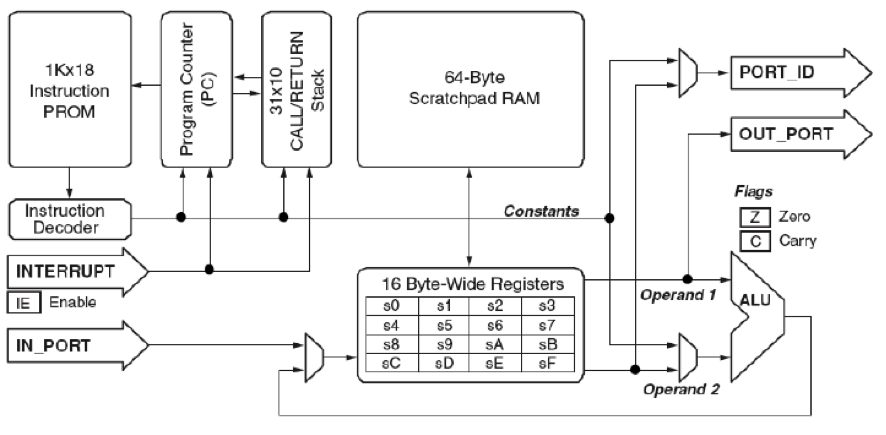
\includegraphics[width=0.8\textwidth,keepaspectratio=true]{./images/estructurapico}
  	\caption{Estructura interna del microcontrolador PicoBlaze}
  	\label{fig:PicoBlazer}
 	\end{center}
	\end{figure}

Aunque está orientado para pequeñas tareas de control más que para ejecutar grandes aplicaciones, se utiliza en varios sistemas multiprocesador.

	\subsection{MicroBlaze}

MicroBlaze es un microprocesador RISC de 32 bits desarrollado por Xilinx para sus FPGAs de las familias Spartan y Virtex. Sigue una arquitectura Harvard con buses de memoria de datos e instrucciones separados. Una de sus principales características es su configurabilidad, pudiendo incluir o excluir una serie de elementos del microprocesador según las necesidades de la aplicación objetivo permitiendo una gran variedad de configuraciones más o menos rápidas y que ocupan más o menos área en la FPGA.

Las características más destacables de este SCP son:    

	\begin{itemize}
	  \item  32 registros de propósito general de 32 bits.
	  \item  Instrucciones de 32 bits, con 3 operandos y 2 modos de direccionamiento.
	  \item  Bus de direcciones de 32 bits.
	  \item  Pipeline configurable de 3 o 5 etapas.
	  \item  FPU,\textit{ barrel-shifter} y multiplicador y/o divisor de enteros opcionales.
	  \item  Caché de instrucciones y caché de datos opcionales.
	  \item   3 interfaces de bus disponibles para conectar distintos tipos de periféricos:
		\begin{itemize}
		  \item  LMB \cite{Etiqueta23}(\textit{Local Memory Bus}): Bus síncrono de alta velocidad utilizado principalmente para conectar los bloques de memoria interna de la FPGA.
	 	 \item  OPB \cite{Etiqueta24}(\textit{On-Chip Memory Bus}) : Bus síncrono utilizado para conectar periféricos con tiempos de acceso variables. Tiene soporte para hasta 8 maestros.
	 	 \item FSL\cite{Etiqueta25} (\textit{Fast Simplex Link}): Canales punto a punto dedicados, para streaming de datos. Dispone de 8 canales, cada uno con un puerto de entrada y otro de salida.
		\end{itemize}
	\end{itemize}

La arquitectura general consiste en una serie de bloques presentados en la figura ~\ref{fig:MicoBlazer}.
		
	\begin{figure}[h!]
 	\begin{center}
  	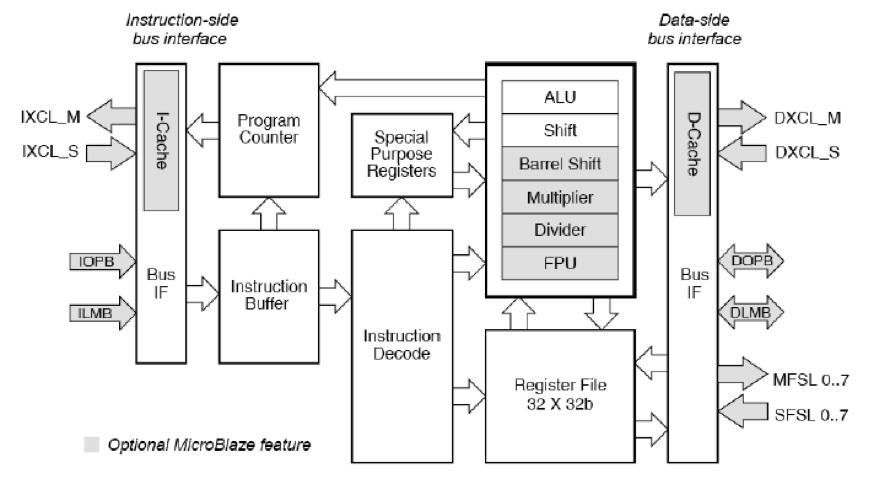
\includegraphics[width=0.8\textwidth,keepaspectratio=true]{./images/estructuramicroblazer}
  	\caption{Estructura interna del microcontrolador MicroBlaze}
  	\label{fig:MicoBlazer}
 	\end{center}
	\end{figure}

Actualmente MicroBlaze es uno de los SCP más utilizado, y parte del éxito se debe
a las herramientas que proporciona Xilinx para crear sistemas basados en este
microprocesador. La herramienta Xilinx Platform Studio\cite{Etiqueta26}permite de forma gráfica e
intuitiva interconectar tanto el procesador como los distintos periféricos y buses que forman
el sistema como se ve en la figura~\ref{fig:Xilinx Platform Studio}

\begin{figure}[h!]
 	\begin{center}
  	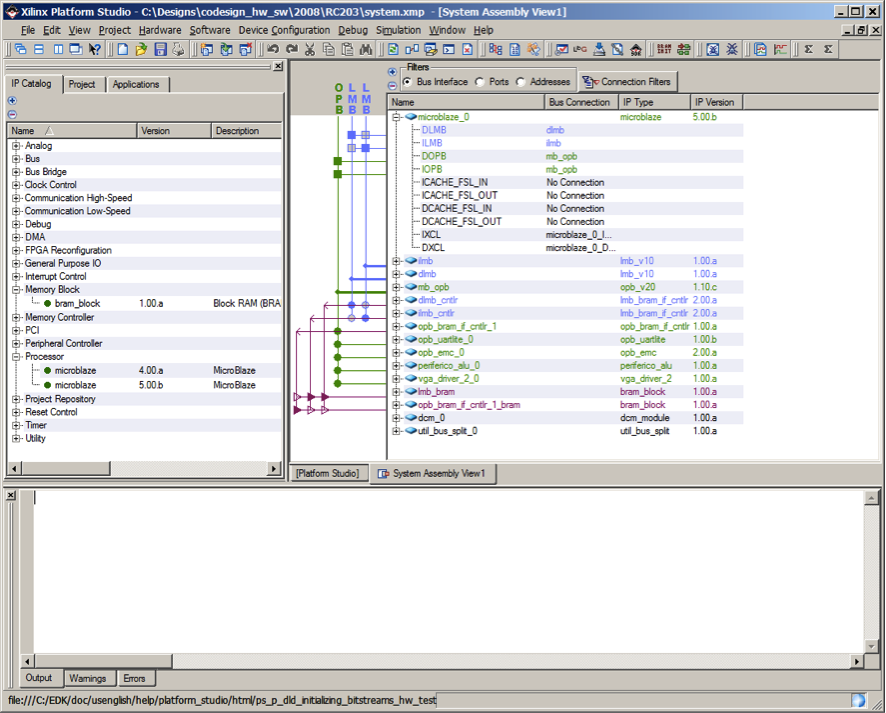
\includegraphics[width=0.8\textwidth,keepaspectratio=true]{./images/herramientaxps}
  	\caption{Interfaz de la herramienta Xilinx Platform Studio}
  	\label{fig:Xilinx Platform Studio}
 	\end{center}
	\end{figure}

También ofrece una bibliotecas de IPs ya diseñadas y listas para integrarse en cualquier diseño como:

		\begin{itemize}
		  \item  Controladores de memoria: SRAM, SDRAM, DDR y DDR2.
	 	 \item  Dispositivos de comunicación serie: bus I2C, UART16550.
	 	 \item Controladores Ethernet y Ethernet Lite.
		\end{itemize}

La herramienta además de ayudar y simplificar la parte de diseño hardware de un sistema basado en el procesador MicroBlaze también ofrece facilidades para el desarrollo de software para el sistema, proporcionando tanto drivers para los distintos periféricos como todo un conjunto de herramientas de desarrollo software (compilador, depurador, bootloader) un micro kernel con interfaz de hilos POSIX y diversas bibliotecas, todo ello integrado en un entorno basado en Eclipse\cite{Etiqueta27} que facilita mucho la tarea del programador de aplicaciones.

	\subsection{Nios II}

Nios II es el procesador que ofrece la compañía Altera para utilizar en sus FPGAs de las familias Stratix y Ciclone. Es un procesador RISC de 32 bits con arquitectura Harvard.

Las principales características de este SCP son:
		\begin{itemize}
		  \item  32 registros de propósito general de 32 bits.
	 	 \item  Operaciones de punto flotante de precisión simple.
	 	 \item  Bus de direcciones de 32 bits.
		 \item  Posibilidad de añadir lógica a la ALU para crear nuevas instrucciones de propósito específico.
 		\item Caché de instrucciones y caché de datos opcionales.
		\end{itemize}
  
Altera ofrece tres versiones diferentes del Nios II, con diferentes características en cuanto a rendimiento y consumo de área.

Las principales características de cada versión del procesador son: 
		\begin{itemize}
		  \item Nios II \textit{fast}: diseñado para ser lo más rápido posible, cuenta con un pipeline de 6 etapas. Incluye operación de multiplicación por hardware en un solo ciclo, previsión dinámica de saltos y cachés separadas de instrucciones y datos.
	 	 \item Nios II \textit{economy}: diseñado para ocupar la menor área posible, ocupa tan solo 700 Logic Elements. Sin caches.
 		\item Nios II \textit{standard}: orientado a aplicaciones de bajo costo, con un rendimiento medio en las aplicaciones. Incluye caché de instrucciones, pipeline de 5 etapas y predicción estática de saltos. También ofrece multiplicador, divisor y desplazador hardware opcionales.
		\end{itemize}

\begin{figure}[h!]
 	\begin{center}
  	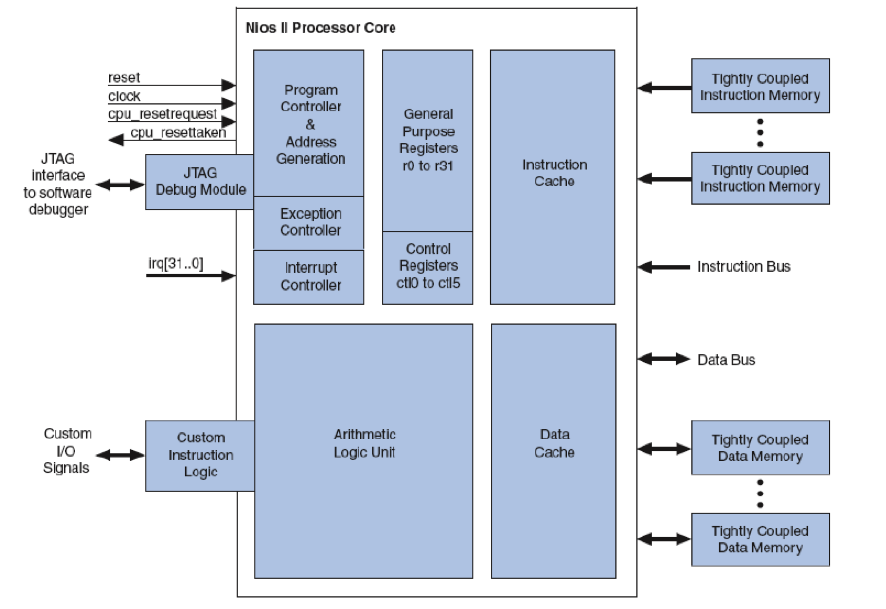
\includegraphics[width=0.8\textwidth,keepaspectratio=true]{./images/nios2}
  	\caption{Arquitectura del procesador Nios II}
  	%\label{fig:Xilinx Platform Studio}
 	\end{center}
	\end{figure}

Al igual que Xilinx, Altera también ofrece una herramienta gráfica que permite crear de forma rápida y sencilla sistemas basados en su microprocesador: System on Programmable Chip Builder \cite{Etiqueta28}figura~\ref{fig:System on Programmable Chip Builder}. También ofrece una biblioteca de componentes como UARTs, dispositivos Ethernet, controladores de memoria, etc, que se pueden integrar a cualquier diseño basado en Nios II.
Además de facilitar la tarea de diseñar la parte hardware del sistema, también ofrece un entorno de desarrollo de software basado en Eclipse que facilita la tarea del desarrollador de software proporcionándole en un único IDE todas las herramientas necesarias como editor, compilador, depurador, bootloader, etc. Además, da soporte para desarrollar aplicaciones que hagan uso del sistema operativo MicroC/OS-II.

	\begin{figure}[h!]
 	\begin{center}
  	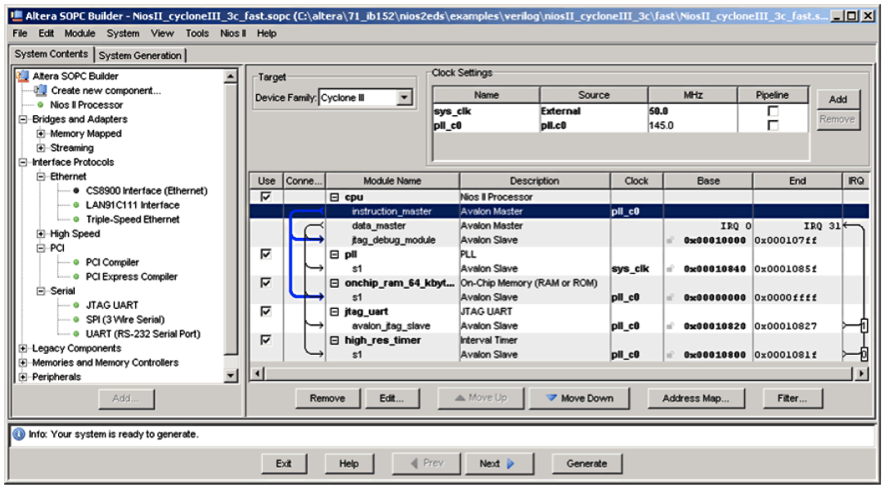
\includegraphics[width=0.8\textwidth,keepaspectratio=true]{./images/herramientasnios2}
  	\caption{Interfaz de la herramienta System on Programmable Chip Builder}
  	\label{fig:System on Programmable Chip Builder}
 	\end{center}
	\end{figure}
\newpage
	\subsection{LatticeMico32}
 
La compañía Lattice ofrece el procesador LatticeMico32 para sus FPGAs. Una de las principales características de este procesador es que, aunque proviene de una compañía privada, se ofrece bajo una licencia libre. Sigue una arquitectura RISC, y utiliza dos interfaces de bus WISHBONE \cite{Etiqueta34}separados para instrucciones y datos.

 El procesador se ofrece en 3 posibles configuraciones con distintas relaciones de área y rendimiento:

\begin{itemize}
		  \item Configuración básica: Sin multiplicador hardware ni cachés. Desplazador multiciclo. Ocupa 1571 LUTs de una FPGA LatticeEC/ECP y puede alcanzar una frecuencia de reloj de 81 MHz.
		 \item Configuración estándar: Con multiplicador hardware, desplazador segmentado y 8 KB de caché de instrucciones. Caché de instrucciones y caché de datos opcionales.Ocupa 2040 LUTS y alcanza una frecuencia de reloj de 89 MHz.
 		\item Completa: Igual que la configuración estándar pero con 8 KB de caché de datos. Ocupa 2230 LUTs y alcanza los 92 MHz.
		\end{itemize}

\begin{figure}[h!]
 	\begin{center}
  	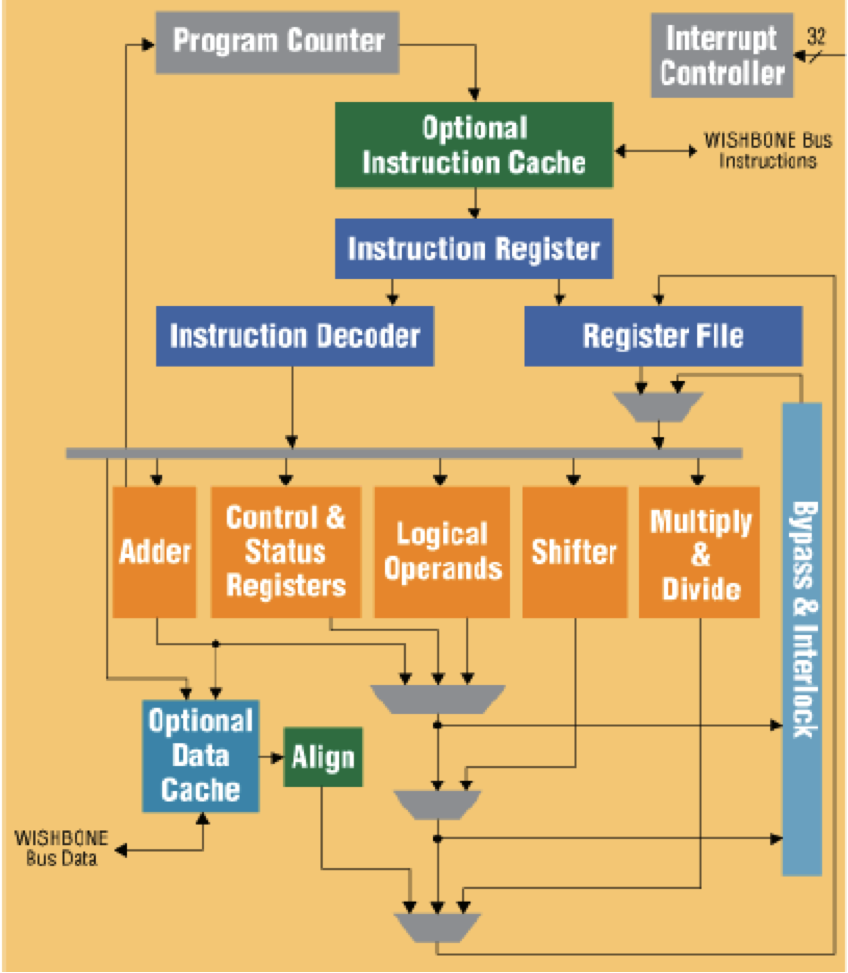
\includegraphics[width=0.5\textwidth,keepaspectratio=true]{./images/latice}
  	\caption{Arquitectura del procesador LatticeMico32}
 	\end{center}
	\end{figure}

Lattice al igual que sus competidoras Xilinx y Altera, ofrece también un entorno de desarrollo para generar sistemas basados en su microprocesador
llamada Mico System Builder figura~\ref{fig:msb}. Desde dicha herramienta permite de forma sencilla interconectar el procesador con los distintos periféricos y buses que
integra la biblioteca de IPs proporcionada por Lattice.

\begin{figure}[h!]
 	\begin{center}
  	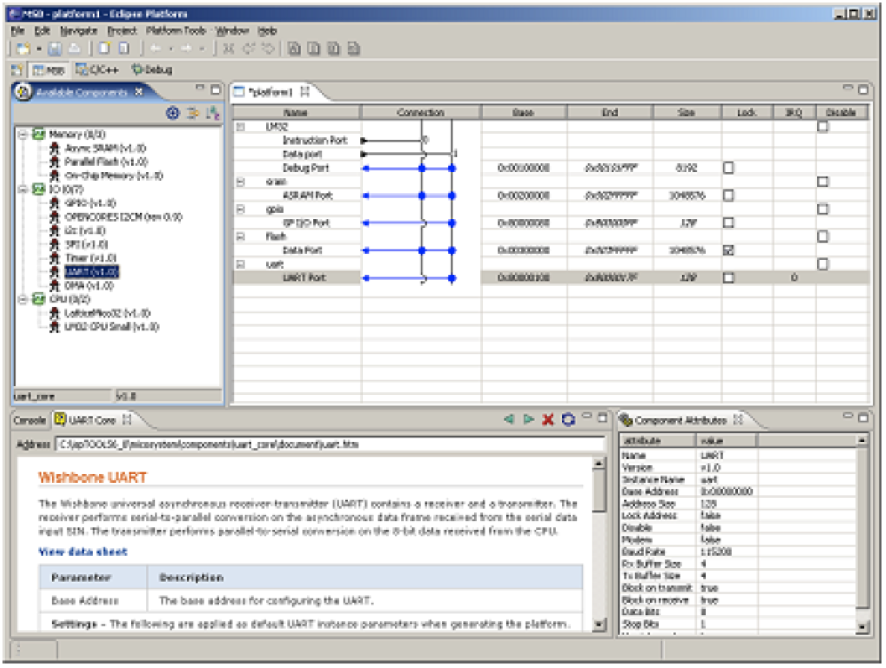
\includegraphics[width=0.8\textwidth,keepaspectratio=true]{./images/herramientaslatice}
  	\caption{Interfaz de la herramienta Mico System Builder}
  	\label{fig:msb}
 	\end{center}
	\end{figure}
\newpage
	\subsection{OpenRISC 1200}

Opencores \cite{Etiqueta20} es una comunidad de hardware de código abierto que ofrece una gran variedad de IPs entre los que se encuentra el microprocesador OpenRISC 1200, un microprocesador RISC de 32 bits que se distribuye como código abierto.

Algunas características de este SCP son:

\begin{itemize}
		 \item  Arquitectura Harvard.
	 	 \item \textit{Pipeline} de 5 etapas.
	 	 \item  Unidad de manejo de memoria (MMU)
		 \item  Cachés de instrucciones y de datos de 8 KB, de mapeo directo.
 		\item Unidades opcionales como: unidad de depuración,\textit{ tick-timer}, controlador de interrupciones y unidad de manejo de potencia (PMU).
		\item Interfaz WISHBONE para los buses de instrucciones y de datos.
\end{itemize}
  
\begin{figure}[h!]
 	\begin{center}
  	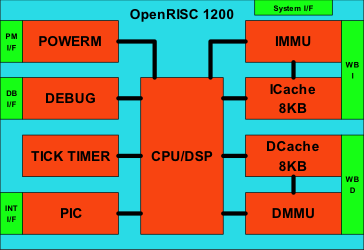
\includegraphics[width=0.6\textwidth,keepaspectratio=true]{./images/OR1200}
  	\caption{Arquitectura OpenRISC}
  	%\label{fig:System on Programmable Chip Builder}
 	\end{center}
	\end{figure}


Las herramientas existentes para desarrollar sistemas basados en el OpenRISC 1200 son muy limitadas y no existe una herramienta similar a las existentes para los procesadores ya comentados que permita interconectar el procesador y los distintos buses y periféricos de una forma sencilla e intuitiva. Existe una herramienta gráfica basada en TCL/TK que permite configurar las diferentes características del procesador de forma sencilla\cite{Etiqueta29}, en lugar de tener que editar a mano el fichero de configuración del microprocesador.

En cuanto a herramientas para el desarrollo de software está también bastante limitado. Se proporcionan las herramientas de compilación y depuración de GNU, y existen también proyectos que mantienen ports de algunos sistemas operativos libres como eCos\cite{Etiqueta30} o uCLinux \cite{Etiqueta31}. Pero no está todo integrado en un entorno de desarrollo ni ofrece las características que ofrecen las herramientas de Xilinx o Altera como generación automática de drivers, generación de scripts de enlazado, generación de BSPs para distintos sistemas operativos.

El rendimiento que ofrece el OpenRISC 1200 es superior al de sus competidores comerciales, a costa de un mayor consumo de área. En \cite{Etiqueta32} se ofrecen diversos datos de comparación de distintos procesadores en distintas configuraciones y se deduce que el área ocupada por un sistema basado en OpenRISC 1200 es entre dos y tres veces superior al de un sistema equivalente basado en MicroBlaze.

   	\subsection{LEON 2 y LEON 3}

LEON 2 es un procesador RISC de 32 bits basado en la arquitectura SPARC-V8\cite{Etiqueta33}. Está desarrollado por Gaisler Research y la Agencia Espacial Europea (ESA). Está completamente descrito en VHDL sintetizable y se distribuye bajo una licencia GPL (General Public License). Algunas de sus características más importantes son:

\begin{itemize}
		 \item  Arquitectura Harvard.
		 \item  Caches de instrucciones y datos configurables.
	       \item \textit{Pipeline} de 5 etapas.
		 \item  Interfaz de bus AMBA.
 		\item  Caché de datos con protocolo \textit{snoop}, que permite coherencia de cachés en sistemas multiprocesador.
		\item Unidad de manejo de memoria (MMU).
		\end{itemize}
	
\begin{figure}[h!]
 	\begin{center}
  	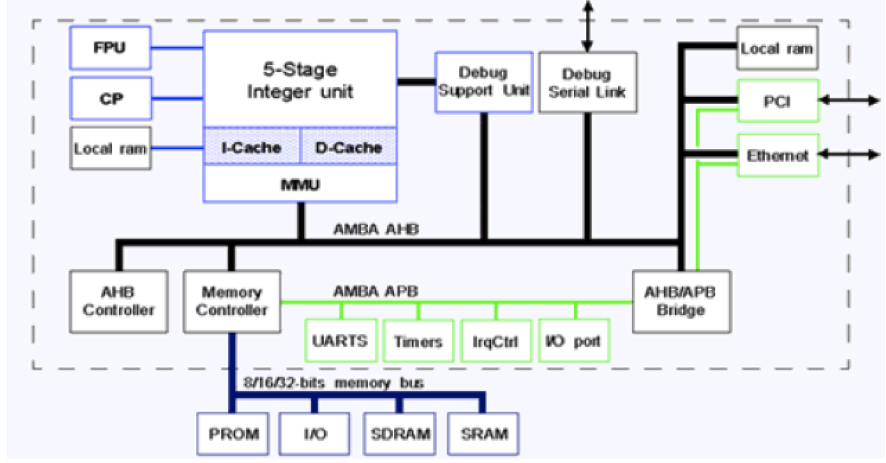
\includegraphics[width=0.8\textwidth,keepaspectratio=true]{./images/leon}
  	\caption{Arquitectura del procesador LEON 2}
  	%\label{fig:System on Programmable Chip Builder}
 	\end{center}
	\end{figure}

Existe una herramienta gráfica que permite configurar las partes opcionales del procesador, pero no existe ninguna herramienta que permita realizar de forma sencilla las conexiones entre buses y periféricos o añadir nuevos periféricos que ofrecen las herramientas comerciales de otros procesadores. En la parte de desarrollo software, Gaisler Research proporciona el compilador LECCS basado en gcc, y un kernel RTEMS de tiempo real. También existen ports de otros kernels como eCos o Linux, mantenidos por terceras partes.

En cuanto a rendimiento LEON 2 es muy superior a todos los procesadores presentados hasta ahora, aunque también es el que ocupa más área: de los resultados que se presentan en \cite{Etiqueta32} se puede ver que en promedio ocupa entre 3 y 4 veces más que un sistema equivalente basado en MicroBlaze y entre 1 y 1,5 veces más que un sistema equivalente basado en OpenRISC 1200. 

LEON 2 ya no tiene soporte y dio paso a LEON 3: un procesador RISC de 32 bits, también compatible con la arquitectura SPARC V8 y que incluye muchas mejoras con respecto a su predecesor:

\begin{itemize}
		 
	       \item \textit{Pipeline} de 7 etapas.
		 \item Unidad de punto flotante completamente segmentada.
		 \item Cachés de instrucciones y de datos mejoradas, hasta 4 veces más grandes.
 		\item  Caché de datos con protocolo \textit{snoop}, que permite coherencia de cachés en sistemas multiprocesador.
		\item Hasta un 50 \% más de frecuencia de reloj.
		\item Soporte para multiprocesamiento simétrico.
		\end{itemize}
   
Todas estas mejoras suponen también un considerable aumento del área necesaria, en torno a un 30 \% más.

